%--------------------------------------------------------------------------------
%\documentclass{article}

\documentclass[a4paper, 12pt]{article}
% \usepackage[T1]{fontenc}
\usepackage[T1]{fontenc}
\usepackage[bf]{caption}
\usepackage[utf8]{inputenc}
\usepackage{graphicx}
\usepackage[czech, english]{babel}
\selectlanguage{czech}
% \usepackage{subfig}                % \subfloat
\usepackage{color}
\usepackage{url}
\inputencoding{utf8}
%\usepackage[bf]{caption2}
\usepackage[right]{lineno}
\usepackage{amsmath}
\usepackage{amssymb}
\usepackage{subcaption}
\renewcommand\linenumberfont{\normalfont\tiny\color{blue}}

\usepackage[unicode,colorlinks,hyperindex,plainpages=false,pdftex]{hyperref}
\usepackage[all]{hypcap}
\hypersetup{
  colorlinks=false,
  linkbordercolor=1 1 1,
  citebordercolor=1 1 1,
  hidelinks
}

\title{Zobrazování volumetrických mraků v pohybu}
\author{Ondřej Janošík <xjanos12@stud.fit.vutbr.cz>}
\date{\today}

%--------------------------------------------------------------------------------


\begin{document}
\selectlanguage{czech}
\maketitle

\section{Úvod}

V~počítačové grafice se ve většině případů kamera nachází pod vrstvou mraků
a zejména pak ve hrách bývají mraky součástí skyboxu,
či simulovány pomocí billboardů. To ovšem nepůsobí dobrým dojmem například
při průletu mraky. Pro tento případ je třeba využít volumetrických dat a právě
zobrazování volumetrických procedurálně generovaných mraků je náplní této práce.

%%%%%%%%%%%%%%%%%%%%%%%%%%%%%%%%%%%%%%%%%%%%%%%%%%%%%%%%%%%%%%%%%%%%%%%%%%%%%%%%%%%%%%%%

\section{Teorie}

V této kapitole popisuji techniky, které lze využít při renderování
volumetrických dat a také způsob generování perlinova šumu.

\subsection{Perlinův šum}

\textit{Perlinův šum} je jednoduše řečeno suma šumů o různých amplitudách
a frekvencích.
Případně lze mezi jednotlivými složkami také zavést fázový posun.
V~počítačové grafice se používá zejména k~dosažení různých efektů,
jako například oheň, kouř, vlnění vodní hladiny nebo také pro generování
terénů či právě mraků a to volumetrických, nebo jen dvourozměrných billboardů.
\cite{url:wiki-perlin-noise}


Základem pro vytvoření perlinova šumu je samotná šumová funkce.
Ta uvnitř ukrývá jednoduchou hashovací funkci.
Hashovací funkce ovšem pracuje pouze s~celými čísly a pro naše potřeby je třeba
šum generovat z~čísel s~plovoucí desetinnou čárkou. Za tímto účelem si získáme
hodnotu šumu v~okolních celočíselných hranicích a na základě desetinné části
interpolujeme (\ref{eq:floating-noise}).
Lze využít například jednoduché lineární interpolace (\ref{eq:mix-lin}),
nebo pak lehce pokročilejší kosinovy interpolace (\ref{eq:mix-cos}), která
má oproti linerání interpolaci hladší průběh. \cite{url:elias-perlin-noise}

\begin{equation}
  \begin{aligned}
    noise(x) & = mix(hash(n_1), hash(n_2), fract(x)) \\
    % where
    n_1 & = floor(x) \\
    n_2 & = n_1 + 1 \\
  \end{aligned}
  \label{eq:floating-noise}
\end{equation}

\begin{equation}
    mixLinear(a, b, x) = a \cdot (1 - x) + b \cdot x
  \label{eq:mix-lin}
\end{equation}

\begin{equation}
  \begin{aligned}
    mixCos(a, b, x) & = a \cdot (1 - x') + b \cdot x' \\
    x' & = \frac{1 - cos(x \cdot \pi)}{2}
  \end{aligned}
  \label{eq:mix-cos}
\end{equation}

Pro získání vzorku $N$-rozměrného šumu je pak třeba získat $2^N$ vzorků
a následně provést $2^N-1$ interpolací. Složitost výpočtu je tedy $O(2^N)$.
Samotný výpočet perlinova šumu pak popisuje
rovnice \ref{eq:perlin-sum}.

\begin{equation}
  \begin{aligned}
    perlin(\vec{x}) & = \sum^{n}_{i=0} noise(\vec{x} \cdot f_i) \cdot A_i \\
    n & \in \mathbb{N} \\
    f_i, A_i & \in \mathbb{R} \\
  \end{aligned}
  \label{eq:perlin-sum}
\end{equation}

\subsection{Ray marching}

\textit{Ray marching} nebo také \textit{volumetric ray tracing} je obrazová
metoda vykreslování volumetrických (objemových) dat.
Zásadní rozdíl oproti klasickému \textit{ray tracingu} je v~tom, že pokud
paprsek narazí na těleso, tak se nezastaví, ale může prostupovat skrze těleso,
většinou s~konstatním krokem, což není podmínkou.
Při tomto průchodu skrze těleso se akumulují různé vlastnosti
jako barva nebo hustota a ty se pak mísí (blendují) do výsledné barvy pixelu
spolu s~pozadím. \cite{url:wiki-ray-marching}

Objemové tělěso je vhodné nějakým způsobem vymezit. Pro tyto účely
lze použít například \textit{bounding box}.

%%%%%%%%%%%%%%%%%%%%%%%%%%%%%%%%%%%%%%%%%%%%%%%%%%%%%%%%%%%%%%%%%%%%%%%%%%%%%%%%%%%%%%%%

\section{Popis řešení}

% Tady stručně popište, jakým způsobem jste prakticky projekt řešili. Uveďte zejména použité
% technologie a algoritmy. Zaměřte se hlavně na zajímavé a důležité části implementace a také na
% problémy, které jste řešili. Není nutné popisovat každou třídu.
%
% Např. uveďte, jak jste matematický popis z předchozí kapitoly implementovali prakticky.

V rámci řešení jsem využil ray marching s podvzorkováním $\frac{1}{8}$,
compute shader a 2D a 4D perlinův šum.
V~první fázi jsem vykreslil oblohu bez mraků a terén. Do textury jsem
si uložil jednak barvu, tak i~vzdálenost fragmentů od pozice kamery. V~tomto
případě se však nejedná o~standardní depth buffer\footnote{
Depth buffer neukládá vzdálenost fragmentu od kamery, nýbrž
nejkratší vzdálenost od roviny kamery. To může vést k~nežádoucím efektům
při pohybu kamery.}.
V~následující fázi jsem spustil compute shader s~podvorkováním kvůli snížení
výpočetní náročnosti. Samotná metoda vykreslení je popsána v~kapiloe \ref{sec:cloud-rendering}.

\subsection{Terén a volumetrická reprezentace mraků}

Při implementaci jsem použil perlinův šum rovnou dvakrát.
Poprvé jako výškovou mapu pro generování terénu, podruhé pro samotné mraky.
Bylo třeba implementovat 2D a 4D\footnote{Čtvrtou složkou 4D šumu je čas.},
perlinův šum.

V~případě 2D šumu jsem si vystačil s~\textit{bikosinovou interpolací}\footnote{
Bikosinova interpolace je podobná interpolaci bilineární, místo
linerání interpolace však používá interpolaci kosinovu (\ref{eq:mix-cos}).
}
která je implementačně relativně jednoduchá. Na~obrázku \ref{fig:interpolation}
popisující $N$-rozměrnou linerání/kosinovu interpolaci si lze všimnout,
že interpolaci v~$N$-rozměrném prostoru je možné vyjádřit jako dvě interpolace
v prostoru o~jednu dimenzi nižším a jednu lineární/kosinovu interpolaci.
Pro generování mraků mi pak posloužil 4D perlinův šum.

\begin{figure}
  \centering
  \subcaptionbox*{Princip bilineární (2D) interpolace.}{
      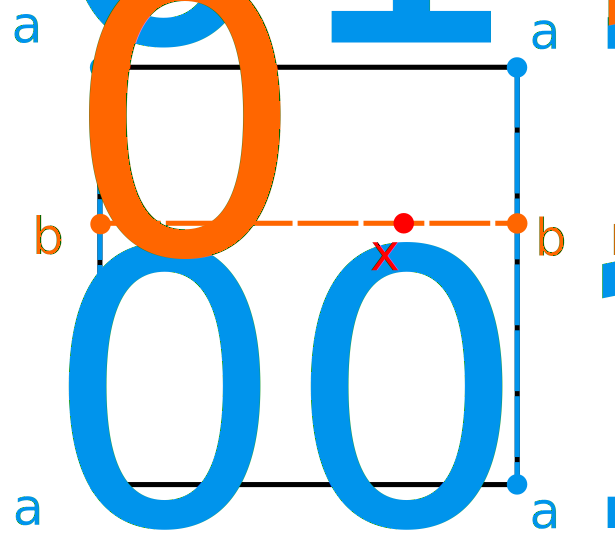
\includegraphics[width=6cm,keepaspectratio]{img/bi-interpolation}
  }
  \hspace{0.5cm}
  \subcaptionbox*{Princip trilineární (3D) interpolace.}{
      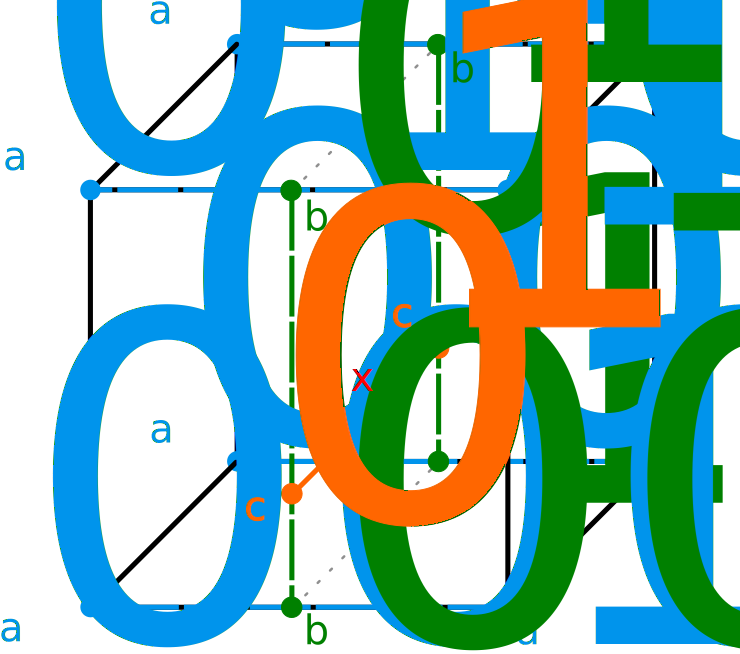
\includegraphics[width=6cm,keepaspectratio]{img/tri-interpolation}
  }  \\
  \vspace{2cm}
  \subcaptionbox*{Princip quadrilineární (4D) interpolace.}{
      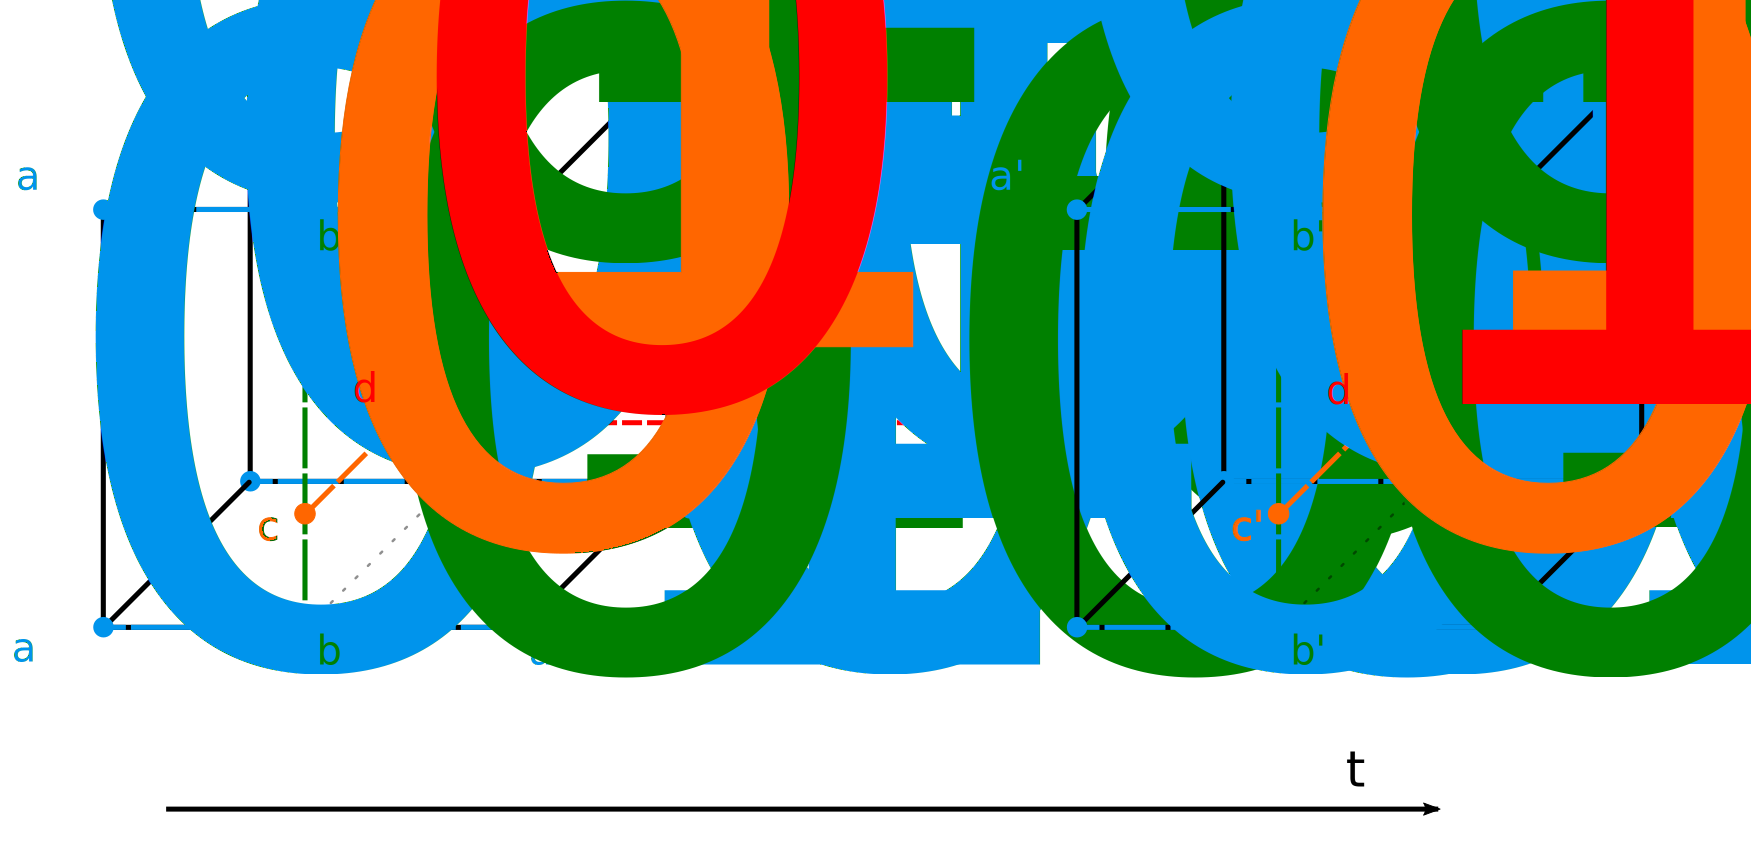
\includegraphics[width=12cm,keepaspectratio]{img/quadri-interpolation}
  }
  \caption{Porovnání $N$-rozměrné linerární/kosinovy interpolace.}
  \label{fig:interpolation}
\end{figure}

\subsection{Vykreslení mraků} \label{sec:cloud-rendering}

U~ray marchingu začínáme stejně jako v~případě ray tracingu a to projekcí
paprsku z~prostoru obrazovky do prostoru scény s~použitím inverzní
view--projekční matice, což je popsáno v~rovnici \ref{eq:unprojection}.
$\vec{r}$ je normalizovaný směrový vektor paprsku a $x$, $y$ jsou
normalizované souřadnice zařízení (\textit{NDC}).

\begin{equation}
  \vec{r} = normalize( (P \cdot V)^{-1} \cdot (x \cdot 2 - 1, y \cdot 2 - 1, 1, 1))
  \label{eq:unprojection}
\end{equation}

Vrstva mraků je vymezena dvěma rovinami rovnoběžnými s~rovinou $y$.
Při projekci paprsku pak teoreticky může dojít k~devíti různým případům
zobrazených na obrázku \ref{fig:camera-possibilities}.
V~mém případě jsou však obě roviny nad úrovní terénu a k~případům $1b$, $2b$ a $3b$
tedy nedojde.

Vzhledem k~tomu, že známe výškové rozmezí v~jaké se mraky nachází, můžeme
dosazením do rovnice \ref{eq:ray-distance} získat vzdálenost oblasti mraků
od kamery (počátku paprsku) a přeskočením této vzdálenosti snižit počet iterací
potřebných k~ray marchingu.

\begin{equation}
  \begin{aligned}
    d & = (y_{clouds} - y_{rayOrigin}) / y_{rayDirection}
  \end{aligned}
  \label{eq:ray-distance}
\end{equation}

\begin{figure}
  \centering
  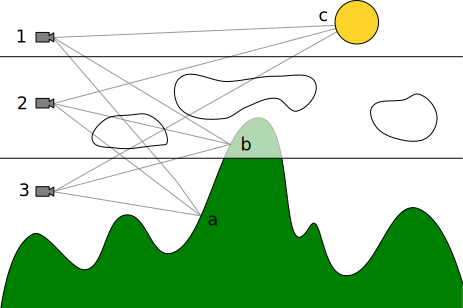
\includegraphics[width=9cm,keepaspectratio]{img/camera-possibilities}
  \caption{Možnosti, které mohou nastat při ray marchingu.}
  \label{fig:camera-possibilities}
\end{figure}

Při průchodu se z~hustoty mraků v~vzorkovaném místě akumuluje průhlednost,
paprskek v tomto případě postupuje stále stejným směrem
(modrá šipka na obrázku \ref{fig:cloud-marching}).
Po překročení práhu průhlednosti $1.0$ je mrak považován za zcela neprůhledný
a iterace je ukončena.

Dále je třeba zjistit světlost mraku. V~ideálním případě bychom vyslali
v~každém vzorkovaném bodě předchozího kroku paprsek směrem ke slunci,
a~kromě akumulace průhlednosti bychom míchali úroveň světlosti.
Pro výpočet v~reálném čase je to příliš náročné a proto je vyslán pouze
jeden paprsek (červená šipka na obrázku \ref{fig:cloud-marching}) směrem ke slunci,
který zjistí kolik světla mrak v~daném místě propouští. Tato aproximace může
v~případě, kdy první paprsek protíná dva mraky přičemž první je částečně průhledný
a světlý zatímco druhý je tmavý. Tmavá barva druhého mraku je nahrazena světlou
barvou mraku prvního.

\begin{figure}
  \centering
  \includegraphics[width=7cm,keepaspectratio]{img/cloud-marching}
  \caption{Výpočet průhlednosti a světlosti mraku.}
  \label{fig:cloud-marching}
\end{figure}

%%%%%%%%%%%%%%%%%%%%%%%%%%%%%%%%%%%%%%%%%%%%%%%%%%%%%%%%%%%%%%%%%%%%%%%%%%%%%%%%%%%%%%%%

\section{Vyhodnocení}

% Tady by mělo být napsané jak to funguje. Protože se jedná o počítačovou grafiku nebo
% vidění, tak by tady měl byt screenshot, ze ktereho bude poznat jak to funguje.
% K tomu by měla být idealně tabulka s vyhodnocením jak přesně/rychle to funguje.

Podařilo se vytvořit algoritmus, který metodou ray marching vykresluje
mraky vygenerované z~4D perlinova šumu. Mraky nevypadají příliš reálně, ale
to už je spíše záležitost nastavení různých parametrů, než zásadními změnami
v~algoritmu.

\begin{figure}
  \centering
  \includegraphics[width=15cm,keepaspectratio]{img/PGP-Clouds-01}
  \caption{Ukázka výstupu aplikace.}
  \label{fig:app-demo}
\end{figure}

Aplikace byla testována na grafické kartě \textbf{nVidia GeForce 680m GTX}.
Na této grafické kartě běžela aplikace při rozlišení $1200 \times 800$ přibližně
rychlostí \textbf{4 snímky za sekundu}, nejedná se tedy o~real-time vykreslování.

%%%%%%%%%%%%%%%%%%%%%%%%%%%%%%%%%%%%%%%%%%%%%%%%%%%%%%%%%%%%%%%%%%%%%%%%%%%%%%%%%%%%%%%%

\section{Závěr}

% Tady by mělo být stručně napsané jak to funguje.

Výsledná aplikace není příliš optimalizovaná. Rozdělením procesu vykreslování
mraků na více fází (uložení šumu do 3D textury, výpočet světlosti v~textuře,
vykreslení mraků průchodem texturou) nebo použitím statických dat by bylo možné
zvýšit rychlost vykreslování a také se zbavit některých nedostatků.

\nocite{url:clouds-wakapon}

\bibliographystyle{czechiso}
\begin{flushleft}
  \bibliography{dokumentace}
\end{flushleft}

%\appendix
%\newpage
%\section{}

\end{document}
